\chapter{The Diffusion of Spices}
\label{ch:diffusion}


% Empirical Chapters
% Discuss and present your findings in a factual way.
% What are the results of your investigations?
% How do the findings relate to previous studies?
% Was there anything surprising or that didn’t work out as planned?
% Are there any themes or categories that emerge from the data?



\lettrine[lines=\iniciale]{\textcolor{\accentcolor}{I}}{n} this chapter, I will present the findings on the diffusion of spices, by looking at the distribution of spice plants and their primary names. First, an overview about the spices' geographical distribution will be presented. Then, a discussion on their spread and \textit{spreadability} will ensue, and lastly, I will present my findings on the diffusion of wandering spice names along spatial and temporal trajectories, and how they relate to the botanical reality. The aim of this chapter is to have an understanding of how spices spread around the globe as informed by their names and etymologies, but at the same time supported by the evidences and current state of their physical diffusion.

\section{The Geographic Distribution of Spices}

\begin{wrapfigure}{R}{0.33\textwidth}
    \vspace{-\baselineskip}
    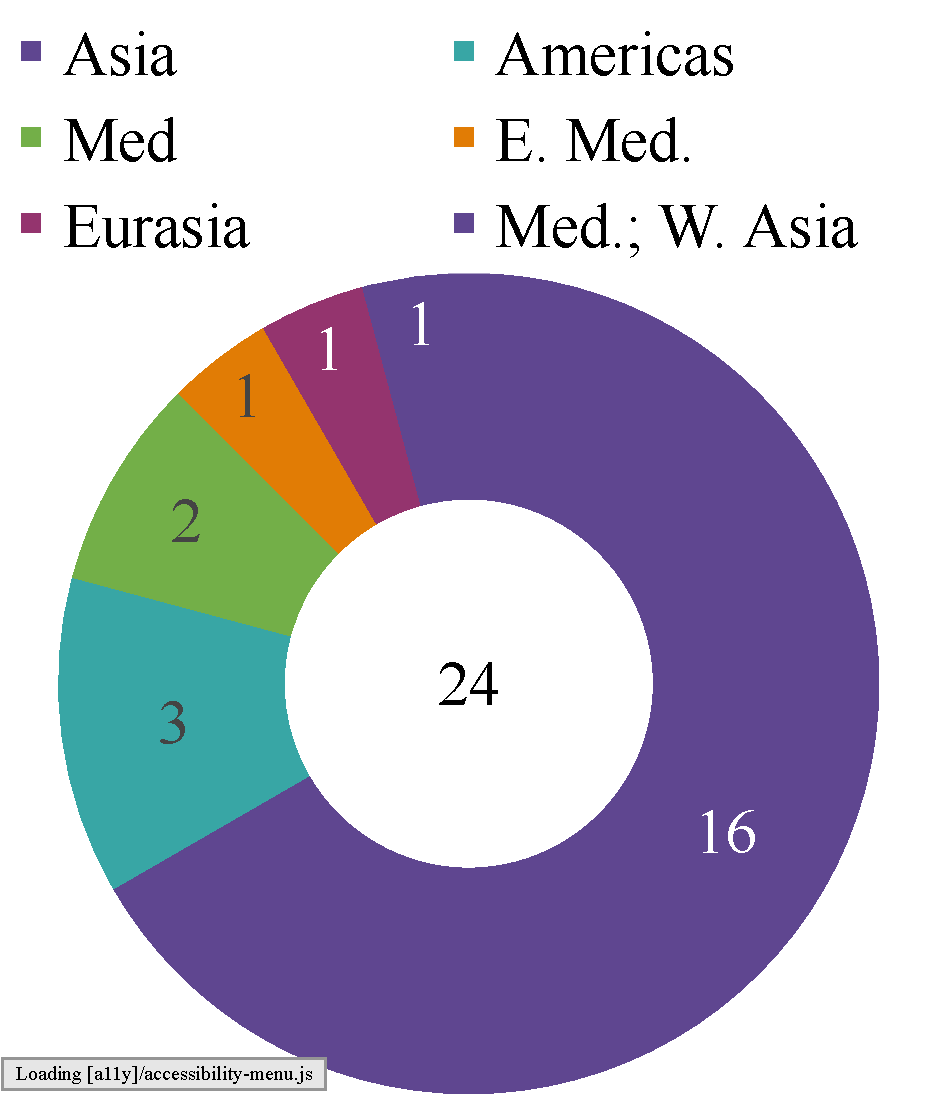
\includegraphics[width=0.33\textwidth]{imgs/plots/macroarea_pie.pdf}
    \caption[Distribution of spice plants by the macroarea of their native habitat.]{Distribution of spice plants by the macroarea of their native habitat.}
    \label{fig:macroarea_pie}
  \end{wrapfigure}
  
In general, it is true that spices come from the hot and humid tropical regions, especially Asia. However, there are number of aromatic plants that originate from more temperate regions, here we should think about the umbelliferous plants of West and Central Asia: asafoetida, fennel, cumin, caraway, and others, and we must not forget the three American spices: chile, vanilla, and allspice. \Cref{fig:macroarea_pie} shows the macroareas where the 24 spices originate.

Botanical databases, such as \gls{POWO}, often show distribution and  give us the regions where a plant is \textit{native} to, and where it has been \textit{introduced}. ``Introduced'' means that the plant is not native in the area, but now grows wild due to human intervention---whether the plant escaped cultivation, or became naturalized after accidental introduction---or due to natural spreading. Looking at this information reflects on the plants' ability to adapt and grow in new places, but also hints on how human usage and transmission affected and created habitats. I have collected this information and used it to compare the spices in question. I have simply counted the native and introduced regions, and added them up. In \cref{fig:total_regions}, you can see the spices ranked by the total number of the regions they grow in, including both native and where the plants were consequently introduced. I would like to highlight that the highest ranks are occupied by aromatic plants that are also herbs, both in the botanical and in the culinary definition. This makes sense, since these plants---e.g., fennel, coriander, dill, fenugreek, etc.---are not only cultivated for their seeds, but the fresh leafy green parts are made use of as well, so it is without question that the whole plant ``travels'' to new places, not only its dried product. Chili peppers are also available fresh in many places today. People transplant their ingredients whenever they can, unless the primary goal of cultivation is purely profit.\footnote{The Dutch for example actively destroyed plant habitats, and wiped out whole islands---including the population---in the Spice Islands of Indonesia to generate scarcity and ramp up value during their monopol rule in the \nth{17} century.}

\begin{figure}[!t]
	\subfloat[Total number of growing regions.]{
	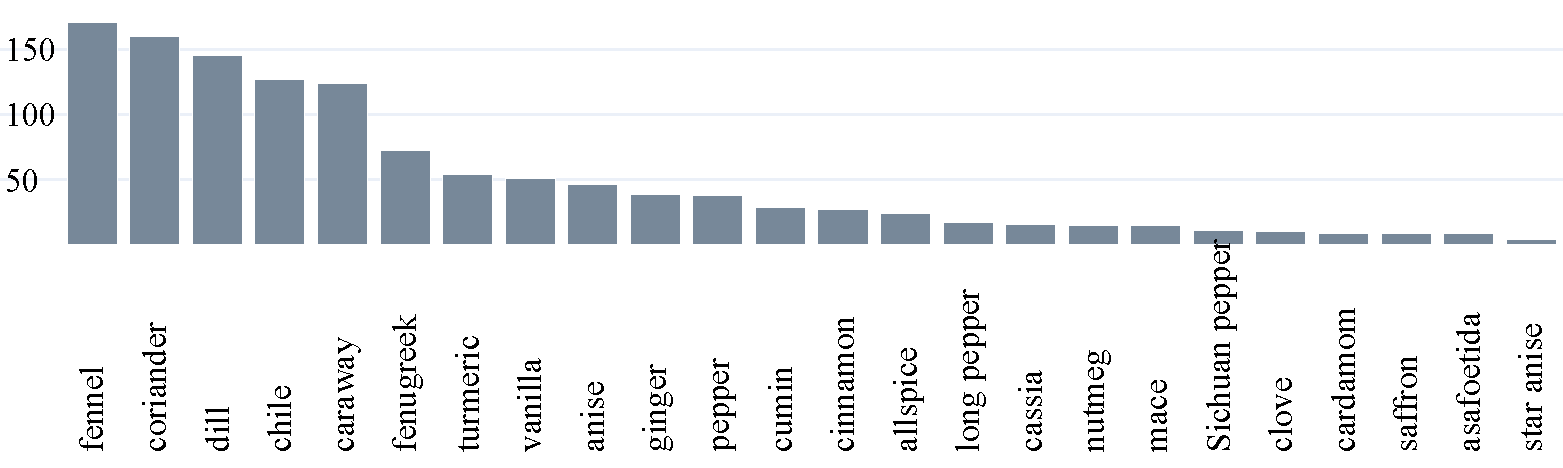
\includegraphics[width=\linewidth]{imgs/plots/total_regions.pdf}}

	\subfloat[Spices by total number of growing regions, grouped by macroarea.]{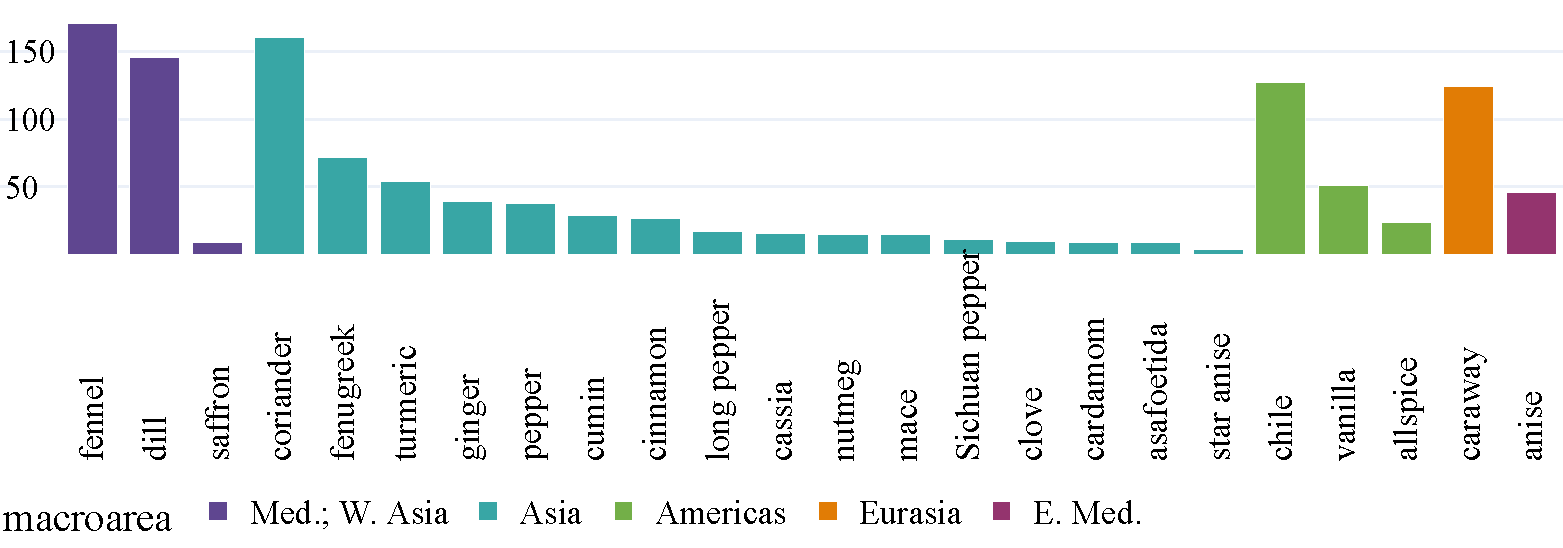
\includegraphics[width=\linewidth]{imgs/plots/total_regions_by_macroarea.pdf}}

	\subfloat[Spices by total number of growing regions, grouped by family.]{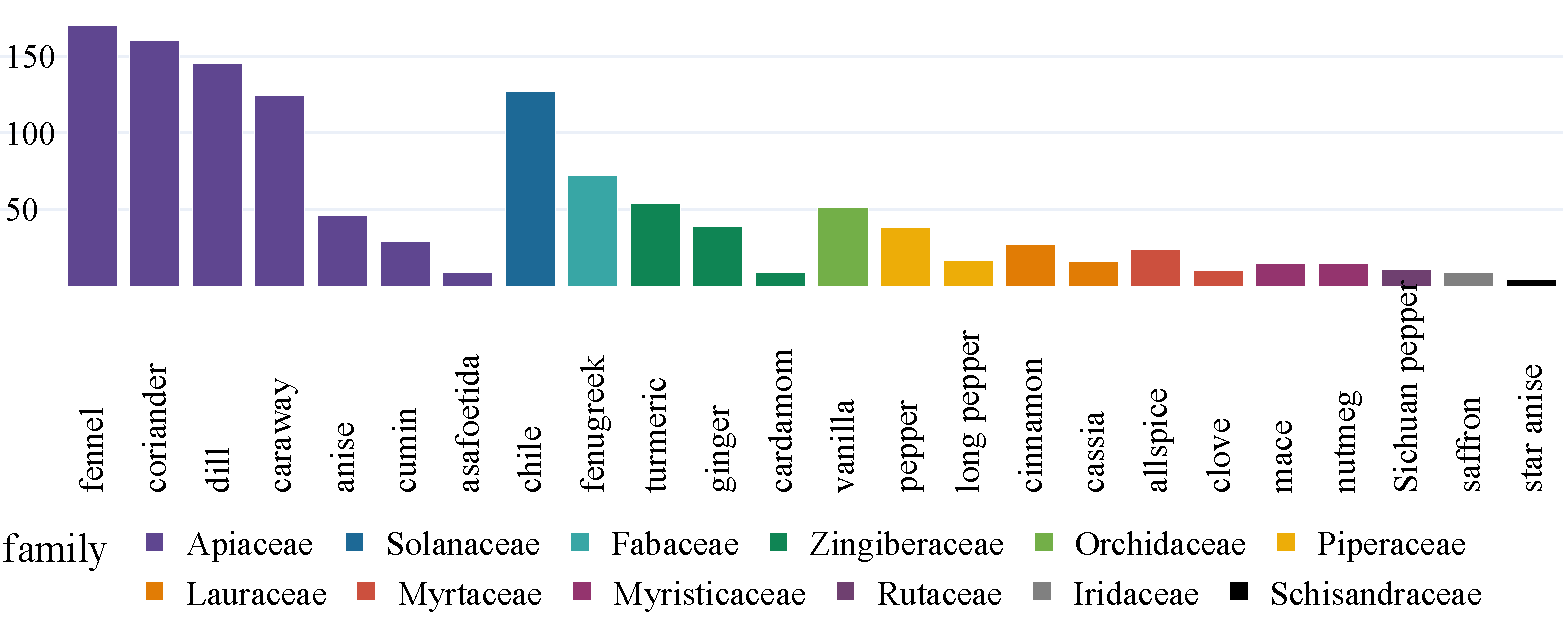
\includegraphics[width=\linewidth]{imgs/plots/total_regions_by_family.pdf}}

	\caption[Spices ranked according to the total number of regions they grow in.]{Spices ranked according to the total number of regions they grow in, both native and introduced.}
	\label{fig:total_regions}
\end{figure}

The far side of the rankings show the spices that do not grow extensively across many regions, regardless of how valuable or popular they are: star anise, asafoetida, saffron, cardamom, cloves. Of course, behind this, are the complex issues of plant biology, ecology and the many factors that decide a plant's resistance to transplantation and if it can grow in new, alien environments. However, there is another point to notice here: labor. The lower ranks feature spices that are highly labor intensive to cultivate and harvest, including star anise, cardamom, and saffron, but the collection of asafoetida is cumbersome as well, and this also effects prices. This seems to indicate that the harder it is to cultivate a spice plant, the less likely it is that it will spread to new places. Interestingly---and of course, closely related what was just said---all of these are products that are very specific plant parts, the pericarps (star anise, Sichuan pepper), dried oleo-gum-resin, (asafoetida), stigmas (saffron), and dried flower buds (cloves). \Cref{fig:total_regions} also shows a grouping by macroarea and by plant family as well.



\subsection{The Spreadability of Spices}
\label{sec:spreadability}

When it comes to spices of commerce, there is a factor that greatly weighs in on their diffusion: their ability to spread. I have noticed that while some spices were very expensive at some point in time (or still are) others, with the same levels of demand, were never particularly costly. Related to the ideas of supply and demand, the answer to this question was scarcity; or in this case, the lack thereof. To put it simply, a spice was expensive if it was rare or its supply was tightly controlled, not unlike diamonds today. Spices that could be easily grown anywhere were transplanted early on and were therefore not considered for their lavish returns, however venerated and influential they were. The two best examples for this are ginger and chili. 

If you have ever left a knob of fresh ginger on you kitchen counter for weeks or even months, you might have noticed that it does not rot, it will eventually sprout and start growing a plant (similarly to an onion or a potato). And if you want more ginger root later, you should put it into a pot of soil. This was the secret of gingers' prehistoric success, which is most known in connection with the Austronesian expansion that began around 5000 years ago, populated the Pacific, and generally believed to have unfurled out of Taiwan \autocite{mirabal_ascertaining_2013}. The early Austronesians carried ginger everywhere on their migrations into Maritime Southeast Asia and the Pacific on their outrigger boats (a native Austronesian invention that enabled people to reach as far as Hawaii and Madagascar), as it was a valuable source of nutrition with added medicinal value \autocite[see][21-25]{dalby_dangerous_2000}. Ginger with its numerous health benefits strengthens the immune system, and was therefore an invaluable crop to carry on long ocean voyages and was a constant feature onboard ships of maritime Asia (compare the ``discovery'' of lemon's effectiveness against scurvy by British naval doctor James Lind in 1747 \autocite{allan_finding_2021}). Accordingly, there is a reconstructed Proto-Oceanic term for ginger, \textit{*laqia} \autocite[52]{bellwood_austronesians_2006}, and a Malagasy term for ginger seems to correspond to a Sanskrit etymon: \textit{sakarivo} < \textit{śṛṅgavera} \autocite[41]{adelaar_malay_1994}. More recent genetic and archaeobotanical studies support the Austronesian expansion theory, which in the past two centuries was solely standing on linguistic grounds. The names of ginger are among the linguistic clues that helped anthropologists, ethnographers, and linguists to reconstructs and establish a chronology. But there is a botanical clue as well that this is a very ancient spice and a long-term product of trade: it is not found in the wild anymore \autocite{ravindran_ginger_2005}. Although it is naturalized in India, it is believed to originate in Southeast Asia \autocite{ravindran_ginger_2005}. The ease of ginger rhizomes' transportation over long distances means that it have spread to other tropical and subtropical regions at a very early time, making the primary center of domestication hard to locate. It was hence called the most widely cultivated spice \autocite{lawrence_major_1984}, which I am almost certain today would be the chili pepper. \textcite{dalby_dangerous_2000} also points out that because humans propagate ginger for millennia by splitting the rhizome, it has lost its ability to be grown from seeds.

Chili on the other hand can reproduce from seeds, and is easy to grow in temperate areas as well. So much so that the American spice became an integral part of many European, African, and Asian cuisines in less then a hundred years since its introduction by the Portuguese, and many often forget that it in fact came from the New World. The red peppers were introduced to Hungary by the Ottomans soon after their conquest marked by the Battle of Mohács in 1526, hence the initial name \textit{törökbors} [turkish-pepper (of \textit{Piper nigrum})], and Hungarian \textit{paprika}---referring to the fine red powder made from dried chilies (attested in 1748, a borrowing from \gls{SCB})\footcite[paprika]{zaicz_etimologiai_2006}---soon came to be an integral part of Hungarian cuisine and identity. Chilies reached Asia soon as well, \textcite{dott_chile_2020} in his well researched book about the cultural history of the chile in China writes that an 1614 Korean encyclopedia noted ``Now it is grown everywhere [in Korea]'', which means it has been introduced to Korea before, and even in 1621, some Chinese \gls{bencao} author believed it to come from Sichuan! ``It comes from central Shu [Sichuan]. Now it is found everywhere.''---reports the \gls{Shiwu} \autocite[24,28]{dott_chile_2020}.

And so, it is clear that some spices spread more easily than others, affecting trade patterns, prices, and the diffusion of names. But how to compare this? How to measure it? To have a basic understanding of what effect spices' ease or difficulty to spread can have on their diffusion, value, and global popularity, I created a rudimentary metric based on geographical-botanical data from \gls{POWO} \autocite{powo}. I will call this \textit{spreadability}. I have simply divided the sum of the introduced regions with the sum of the native regions to serve as a crude indicator of how \textit{well} a spice plant have spread. Intuitively, this index is about spice plants' ability and ``ecological willingness'' to spread to new regions, whether it is a result of human hands (by trade and transplantation) or nature (self-seeding, spread by birds, etc.) into neighboring areas. 

\[ \frac{\sum region_{introduced}}{\sum region_{native}} = spreadability~index \]

\noindent This metric accounts for the initial difference between if a spice was minimally distributed (i.e.,only found in one or two regions), or well distributed before being introduced to either a few, or many new places. \Cref{fig:spreadability} shows the spices ranked by their spreadability index. The figure shows for example tumeric, originally from ``one region'' (India), is now found in 53 other regions, resulting in the highest score of 53. On the far side of the plot, we can find Sichuan pepper, whose main source, \textit{Zanthoxylum bungeanum} is indigenous to 10 geographical zones in China, but only have been introduced to one region (Uzbekistan), getting a low score of 0.10.



\begin{figure}[!ht]
	\subfloat[Spices ranked by spreadability.]{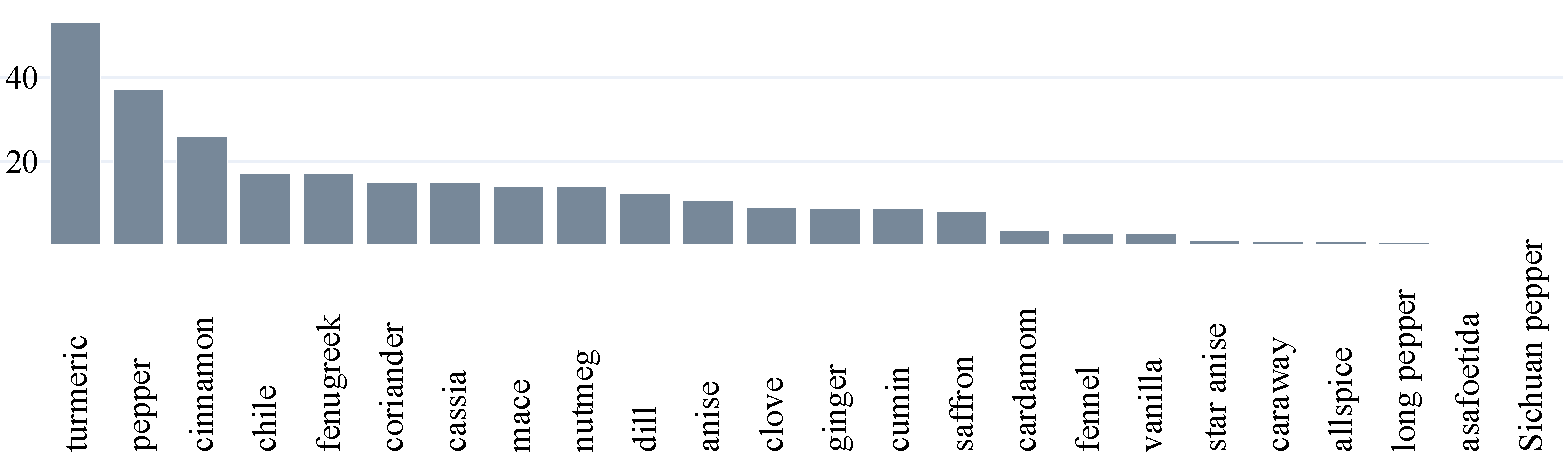
\includegraphics[width=\linewidth]{imgs/plots/spreadability.pdf}}

	\subfloat[Spices ranked by spreadability, grouped by macroarea.]{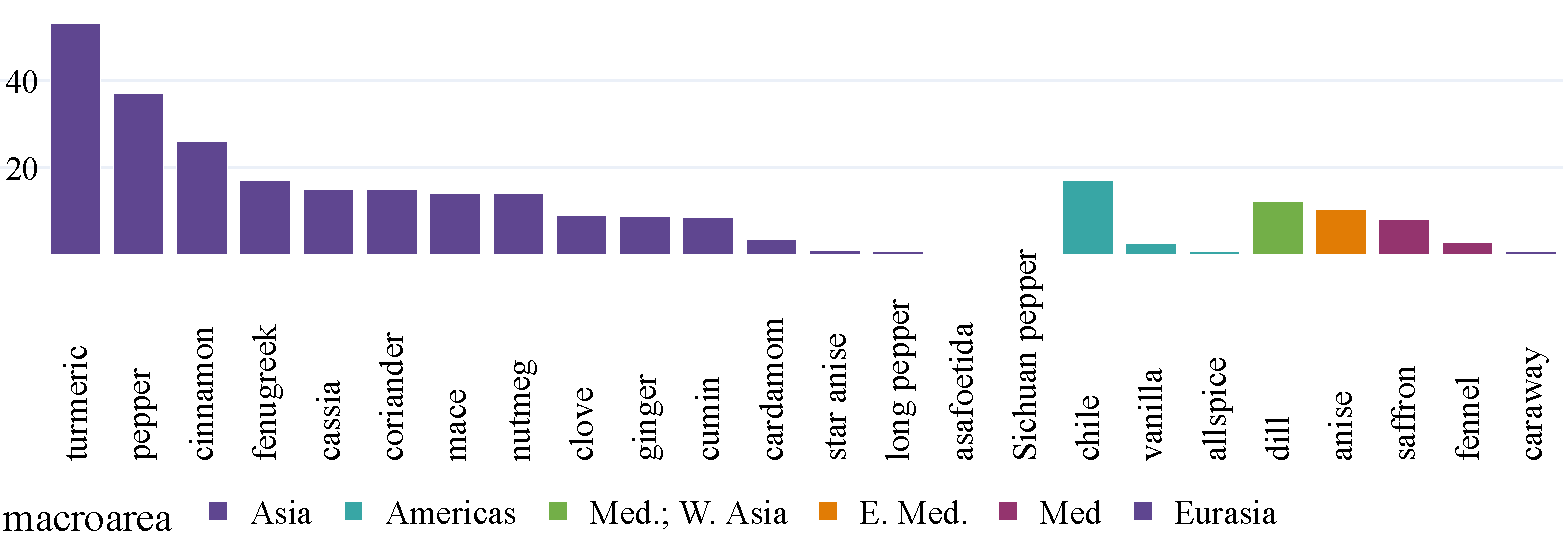
\includegraphics[width=\linewidth]{imgs/plots/spreadability_by_macroarea.pdf}}

	\subfloat[Spices ranked by spreadability, grouped by family.]{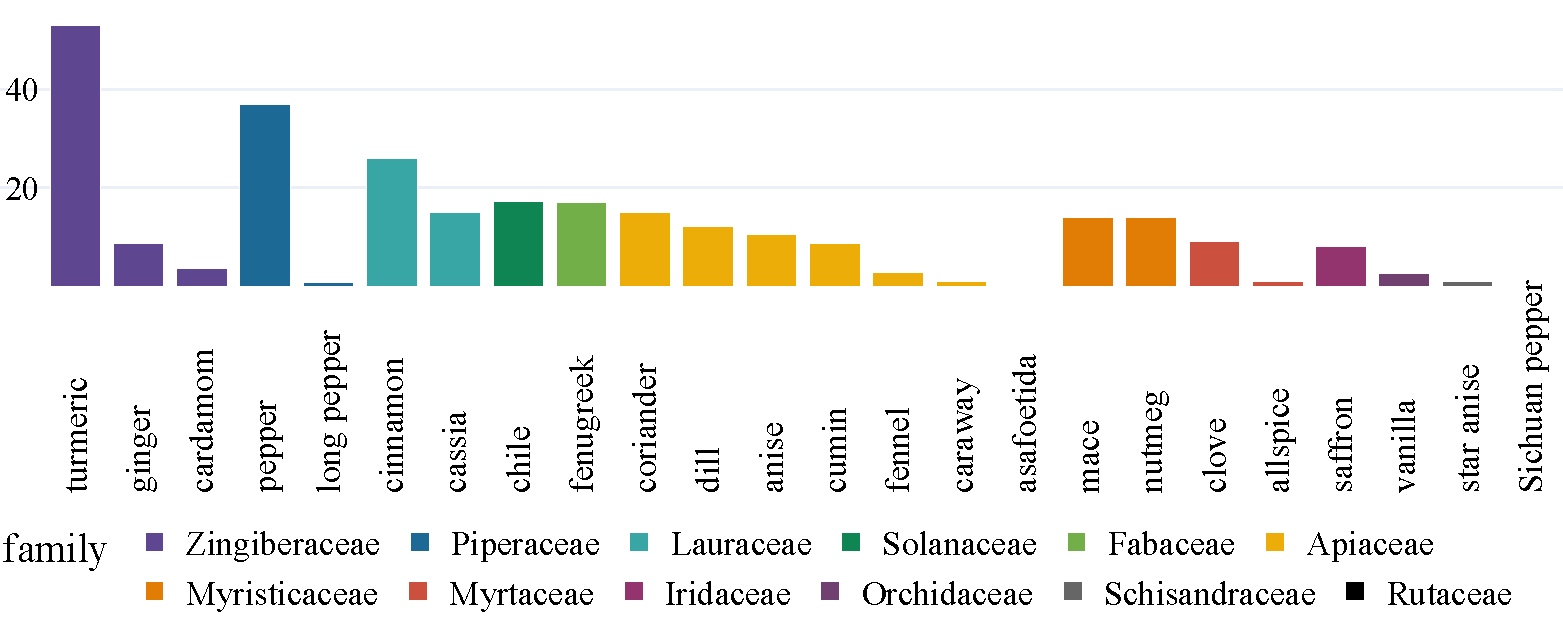
\includegraphics[width=\linewidth]{imgs/plots/spreadability_by_family.pdf}}

	\caption[Spices ranked by their spreadability index.]{Spices ranked by their spreadability index, showing which spice plants spread to more regions, taking into account the initial state of their distribution.}
	\label{fig:spreadability}
\end{figure}



\begin{figure}[ht!]
  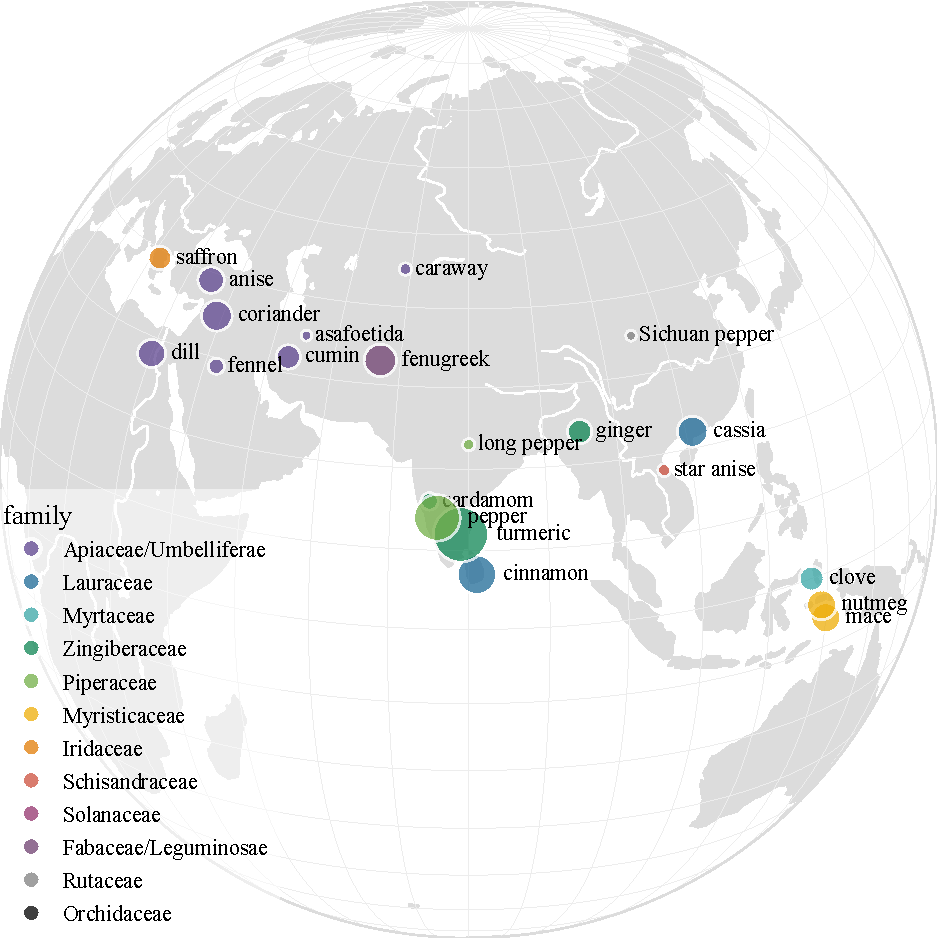
\includegraphics[width=\linewidth]{imgs/plots/distribution_with_spreadability.pdf}
  \caption[The approximate geographical origins of the spices in this thesis.]{The approximate geographical origins of the spices in this thesis; size represents their spreadability index. For a full, interactive version, please visit \url{https://htmlpreview.github.io/?https://github.com/partigabor/phd-thesis-viz/blob/main/spices_map.html}}
  \label{fig:spices_map}
\end{figure}



The results of this graph---like any other---greatly depend on the data we feed to it, and like any other quantitative analysis, has its limitations. Although the regions in the \gls{POWO} database are uniform, they are not clear-cut ecological zones, but rather based on administrative divisions of countries, and it is not perfect. While some large countries are divided to broad areas that represent different biodiversity zones, the borders are arbitrary. For example, the United States, Australia, Russia, and China are divided by states, provinces, or greater geographical areas (e.g., New South Wales, Central European Russia, China South-Central) India is just one unit, explaining the very high score of turmeric.\footnote{Another limitation might be the age of this database as we find zones named Yugoslavia, or Czechoslovakia, but I doubt the biodiversity changed as much as political borders.} Nonetheless, in terms of general usefulness the index has some merit. If we look at the distribution map of turmeric,\footnote{\textit{Curcuma longa} on \gls{POWO}: \url{https://powo.science.kew.org/taxon/796451-1\#distribution-map}} we will see that it did indeed spread far and wide, from Southeast Asia through West Africa to the Caribbean, and compared with Sichuan pepper\footnote{\textit{Zanthoxylum bungeanum} on \gls{POWO}: \url{https://powo.science.kew.org/taxon/775625-1/\#distribution-map}}---which is still mostly limited to China---is much more popular globally. \Cref{fig:spreadability} (b) and (c) show the spices ranked by their spreadability index as well, but broken down by macroarea and plant family. I have included the plant family groupings because it can be very interesting to those with affinity to the plant sciences, but truthfully, this particular grouping would be much more exciting when including more plants in these analyses. 







Based on my readings and data from the botanical databases, I have tried to approximate the geographical origins of each spice in the thesis. \Cref{fig:spices_map} shows this attempt, plotted onto the globe. In cases, where a spice's supposed native area includes a large number of expansive regions, I have opted for a geospatial mid-point as a compromise. Therefore, you can see caraway placed in the middle of Eurasia, because I used the coordinates for Eurasia, as it it is marked native everywhere in Eurasia in the database. Most spice plants \textit{fortunately} do not have so extensive native areas, and in many cases the exact origins can be pinpointed. For example, see the case of nutmeg and cloves neatly situated on tiny islands of the Moluccas in present day Indonesia. %The other side of the globe hides the three spices from the Americas.
The size of the data-points correspond to the their spreadability values, and they indicate very clearly that South Asian spices had a tremendous ``success'' in terms of global diffusion. This also conforms to historical facts; during the centuries old maritime trade between East and West whose two main end points were the entrepôts of Arabia and the port cities of South China, India was the halfway point. Because of its central location of the Maritime Silk Road, it was on the shores of South India where Arabs, Persians, Southeast Asians, Chinese, and later Europeans exchanged goods with each other, and therefore this region was a key point in the spread of spices as well.

What we can know about the diffusion of spices beyond the botanical and historical evidence, is in their names. In most cases, the spice names spread with the materials, and have left a trace. Moreover, these linguistic traces---together with the close study of their respective materials---can help us match or reconstruct the exact routes the materials took, accounting for communities and cultures that have played important roles in their dissemination. The following section will focus on this phenomenon.

\section{The Linguistic Diffusion of Spices}
\label{linguistic_diffusion}

At last, turning towards the language element of spice diffusion, I will now illustrate the linguistic diffusion through the investigation of spice terminology and their spread on spatial and temporal dimensions by tracing loanwords and analyzing attestation timelines. Before introducing the etymological findings, I must touch upon the terms' borrowed status, which I have previously introduced briefly in \cref{sec:borrowed}. Accordingly, this chapter focuses on the borrowed elements of spice terminology.

% \setlength{\tabcolsep}{3pt}

\begin{table}[ht]
    \begin{tabular}{@{}rlclclc@{}}
    \toprule
    \textbf{\#} & \textbf{English} & \textbf{Borrowed} & \textbf{Arabic}  & \textbf{Borrowed} & \textbf{Chinese} & \textbf{Borrowed} \\ \midrule
    1           & allspice         & -           & fulful ifranjī   & -           & duōxiāngguǒ      & +           \\
    2           & anise            & +           & anīsūn           & +           & huíqín           & -           \\
    3           & asafoetida       & +           & ḥiltīt           & +           & āwèi             & +           \\
    4           & caraway          & +           & karāwiyā         & +           & gělǚzi           & +           \\
    5           & cardamom         & +           & hāl              & +           & dòukòu           & ?           \\
    6           & cassia           & +           & salīkha          & -           & ròuguì           & -           \\
    7           & chili            & +           & fulful ḥārr      & -           & làjiāo           & -           \\
    8           & cinnamon         & +           & qirfa            & -           & xīlánròuguì      & +           \\
    9           & clove            & +           & qaranful         & +           & dīngxiāng        & -           \\
    10          & coriander        & +           & kuzbara          & +           & yánsuī           & -           \\
    11          & cumin            & +           & kammūn           & +           & zīrán            & +           \\
    12          & dill             & +           & shibithth        & +           & shíluó           & +           \\
    13          & fennel           & +           & shamar           & +           & huíxiāng         & -           \\
    14          & fenugreek        & +           & ḥulba            & -           & húlúbā           & +           \\
    15          & ginger           & +           & zanjabīl         & +           & jiāng            & -           \\
    16          & long pepper      & +           & dārfilfil        & +           & bìbō             & +           \\
    17          & mace             & +           & basbās           & +           & ròudòukòugānpí   & -           \\
    18          & nutmeg           & +           & jawz al-ṭīb      & +           & ròudòukòu        & -           \\
    19          & pepper           & +           & fulful           & +           & hújiāo           & -           \\
    20          & saffron          & +           & zaʿfarān         & +           & fānhónghuā       & -           \\
    21          & Sichuan pepper   & +           & fulful sītshuwān & -           & huā​jiāo         & -           \\
    22          & star anise       & -           & yānsūn najmī     & -           & bājiǎohuíxiāng   & -           \\
    23          & turmeric         & +           & kurkum           & +           & jiānghuáng       & -           \\
    24          & vanilla          & +           & fānīliyā         & +           & xiāngcǎo         & -           \\ \bottomrule
    \end{tabular}
    \caption[Spice nomenclature, showing if the terms are borrowed or not.]{Spice nomenclature, showing if the terms are borrowed (+), not borrowed (-), or maybe borrowed (?).}
    \label{table:borrowings}
    \end{table}

%   \setlength{\tabcolsep}{6pt}

\begin{figure}[ht!]
  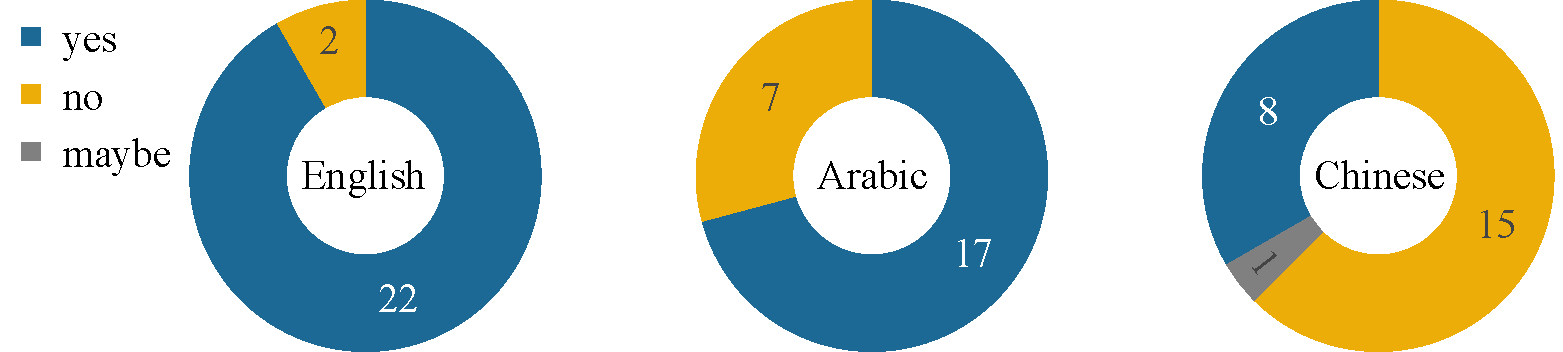
\includegraphics[width=\linewidth]{imgs/plots/borrowing_pie.pdf}
  \caption[{Ratio of borrowed and not borrowed terms in the spice nomenclature.}]{Ratio of borrowed terms in the spice nomenclature across the three languages, based on \cref{table:borrowings}.}
  \label{fig:borrowing_pie}
\end{figure}

\subsection{Borrowings: Loanwords and \textit{Wanderwörter}}

In order to accurately compare the itineraries of loanwords and \glspl{wanderwort} in a trilingual setting, I had to determine which spice names are in fact borrowed, and which are native derivations/inventions. In most instances, it is rather obvious if a word is a borrowing or not, while in others, it was not so easy to determine. For example, I initially assumed that \textit{Sichuan pepper} (which does not occur in English dictionaries) is an English construction and therefore not a borrowing, but after trying to find its source, I learned that it is a calque (loan translation) from Chinese \zh{川椒} \textit{chuanjiao} [Sichuan pepper]\footnote{Which uses the prototype spice word in Chinese, prefixed with the second character of Sichuan province (originally meaning `river').}, devised in the field of herbal medicine \autocite[140]{hooper_chinese_1929}. In short, I analyzed the names based on their borrowed status to find loanwords. The result of this analysis on the default names of the 24 spices can be seen in \cref{table:borrowings}.

The most important finding is that English has by far the most loaned terms in the spice domain---according to our modest sample of spices---followed by Arabic, and finally Chinese. Out of the 24 default names, there are 21 borrowings in English, 17 in Arabic, and 8 in Chinese. \Cref{fig:borrowing_pie} show the ratio of borrowings concisely. Of course, this figure alone can be misleading, since the difference in ratio between the languages is not representative only of the spice domain; the English lexicon has a large number of loanwords in general. Dictionaries especially have a high amount of loanwords, but everyday communication features them greatly as well. For example, out of the top 1000 most frequent words in the \gls{BNC}, more than half are borrowed (usually from French and Latin) \autocite[38]{durkin_borrowed_2014}. We should always approach the percentage of loanwords in a language with caution and I will not cite numbers, but from my studies I know that the percentage of loanwords in English is certainly higher than it is in Arabic, and Chinese, which \textit{prefer} to coin words using native elements. 



Word formation in Arabic most often happens internally by utilizing the possibilities of the highly productive root system, but it seems that in the spice domain, loanwords entered the Arabic vocabulary at high rates as well. Thankfully, the semitic root system and the rules of Arabic word patterns make it easy to spot loanwords. For example, if we take the words \textit{zanjabīl} `ginger', \textit{zaʿfarān} `saffron', or \textit{qaranful} `cloves', we can be sure that these are loanwords for the following reasons: There are no native quinqueliteral (five letter/consonant) roots in Arabic, the few existing ones are borrowings. Furthermore, there are no true ``broken plural'', or related verbal forms for these words. Interestingly, a large amount of Persian (and other) loanwords in the domain of plants, fruits, and vegetables have five-consonant roots, including eggplant, cauliflower, parsley, and oranges.

My knowledge on Chinese word formation is rather limited, but I would like to point out a few phenomena. Firstly, it is well known that while Classical Chinese operated with monosyllabic, single-character words, modern Chinese has a strong tendency to prefer disyllabic words, mainly to to disambiguate homophones. Therefore, only the most ancient spices would have a monosyllabic ancestor, Sinograms that convey the meaning of the spice on their own (e.g., \textit{jiao} `pepper', \textit{jiang} `ginger', \textit{gui} `cassia'). In modern Chinese, ginger is the only one that still can stand alone, pepper and cassia are always affixed with modifiers to distinguish them from other items, and to fit the disyllabic trend. Loanwords will also often conform to this trend and become disyllabic in Chinese when integrated (e.g., \textit{awei} `asafoetida', \textit{bibo} `long pepper', \textit{ziran} `cumin'). Tri-syllabic loanwords are often historical in this domain and not a common feature in day-to-day usage; they are not an integral part of the conventionalized vocabulary (e.g., \textit{zafulan} `saffron' \textit{huluba}, `fenugreek', \textit{geluzi} `caraway'). Secondly, I want to highlight the curiosity of phono-semantic matching. In Chinese, loaned elements are sometimes incorporated by words that are phonetically similar and semantically related, thus hiding the word's or morpheme's borrowed quality. For example, \textit{husui}, a name for coriander literally meaning `barbarian coriander' is supposed to be a phono-semantic matching of an Iranian term (*koswi, *košwi, *gošwi
), according to \textcite{laufer_sino-iranica_1919}.  
% doukou
% is the incorporation of a word into one language from another, often creating a neologism, where the word's non-native quality is hidden by replacing it with phonetically and semantically similar words or roots from the adopting language. Thus, the approximate sound and meaning of the original expression in the source language are preserved, though the new expression (the PSM) in the target language may sound native. 
I will discuss the naming of newly introduced items in more detail in the next chapter.

The fact that English has many loanwords in the spice domain is not surprising if we consider that all of these aromatic products are \emph{exotic}, they are not from anywhere near England, or the Saxon homeland. As for Arabic, we know from the history of the spice trade that virtually all materials from Asia passed through the Arabian Peninsula, and the names of many spices with origins in West Asia predate the Arabic expansion of the \nth{7} century and therefore in Arabic, many are loanwords from other Semitic languages. Loanwords in Chinese in the spice domain are much fewer in number, with most of the historic words being Silk Road terms, or contemporary creations for those introduced in modern times. 

%loanwords in Arabic

%loanwords in Chinese

\subsection{Spatial Trajectories: Tracing Spice Terms Around the Globe}

In order to present the findings in a convenient, reader friendly, and interesting way, I turned to geospatial mapping. The plots seen in this section are made possible by utilizing the etymological data on spice terminology, collected and introduced for each spice in \cref{ch:data}, and justified in \cref{sec:collecting_etymologies}. When creating these visualizations, I have included relevant historic names beyond the 24 default terms such as \textit{amomum}, \textit{dārṣīnī} `cinnamon', or \textit{xingqu} `asafoetida', and I have also left out terms that are not borrowings. Therefore, you will not find words on the plots such as \textit{allspice}, \textit{qirfa} `cinnamon', or \textit{hujiao} `black pepper'.


\begin{note}
  The geospatial plots in this section (fig. \ref{fig:diffusion_en}, \ref{fig:diffusion_ar}, and \ref{fig:diffusion_zh}) are a static version of interactive graphs available online via clicking the links given in the captions. I highly recommend examining these visualizations, as they supply further details on the words' histories, and most importantly, the traces can be isolated by double clicking on an item in the legend, allowing for a clearer view and comparisons. The color palette in these plots does not have any significance, their sole purpose is to visually separate the traces of the terms.
\end{note}

\subsubsection{Spices Flow Into Europe: The Case of English}

\begin{figure}[ht!]
  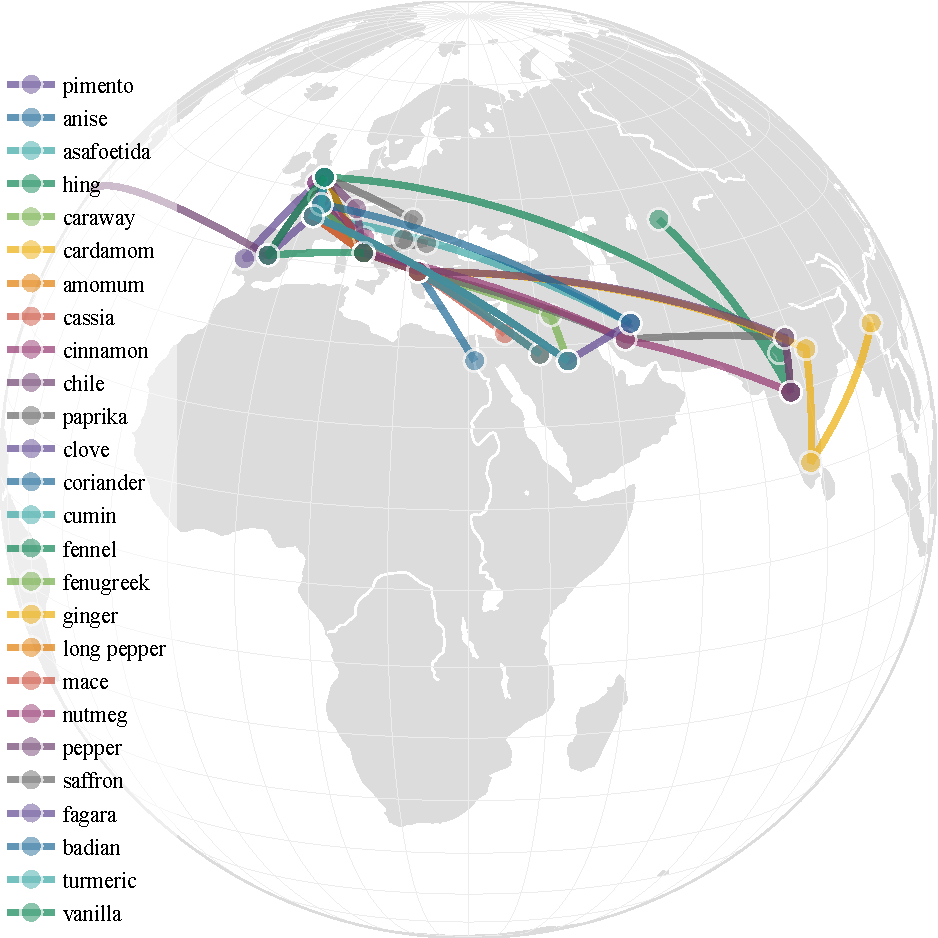
\includegraphics[width=\linewidth]{imgs/plots/diffusion_en.pdf}
  \caption[The diffusion of spice terminology in English.]{The diffusion of spice terminology in English, focusing on loanwords and Wanderwörter. For a full interactive version, please visit \url{https://htmlpreview.github.io/?https://github.com/partigabor/phd-thesis-viz/blob/main/diffusion_en.html}}
  \label{fig:diffusion_en}
\end{figure}

\Cref{fig:diffusion_en} shows the diffusion of spice names viewed from the progression of the words' etymological stages into English. Words that were coined in English (i.e.,not loanwords), are not present. What we see here, is a very clear trend in the dispersion of English spice terminology to have an East-to-West directionality. Besides the few spices that came from the Americas, all via Spanish (\textit{chili}, \textit{pimento}, \textit{vanilla}, where \textit{chili} is represented by the single line crossing the Atlantic Ocean pointing to a Nahuatl etymon) after the \nth{15} century, the majority of spice terms are oriental in origin, and have long histories reaching into times of antiquity and beyond. 

As far as space and distance goes (and probably time as well), the most remote \gls{wanderwort} seems to bee \textit{ginger}, whose source can be traced back to a Dravidian language of South India, but even that form has been identified as a loanword from an unknown Southeast Asian language\footcite[ginger]{oed} (cf. Etmology \ref{ety:ginger}). Based on the cognates in surrounding unrelated languages (Khasi, Thai, Old Chinese), we can assume that ginger in a very early \gls{wanderwort} of the region going back to a Proto-Tibeto-Burman reconstructed form, /*kjaŋ/ \autocite[302]{matisoff_handbook_2003}. Even more exciting is the fact that besides English, the Arabic and Chinese words for ginger originate in the same etymon as well. I recommend using the link to explore the interactive visualization and isolating the trace for ginger, or any other spice, as it is much more clear to inspect a single item as opposed to a crowd.

\begin{etymology}\label{ety:ginger}
English \textit{ginger}, ca. 925
< reinforced by Old French \textit{gingivere, gingibre } `ginger'
< Medieval Latin \textit{gingiber} `ginger'
< Latin \textit{zingiber} `ginger'
< Ancient Greek {\gr{ζιγγίβερις}} \textit{ziggiberis} `ginger'
< Pali \textit{siṅgivera } `ginger'; cf. cognates Sanskrit शृङ्गवेर \text{śṛṇgavera}
< Dravidian \textit{*cinki-wēr} `ginger', South dravidian nominal compound  from the etyma of Tamil and Malayalam \textit{iñci} (both with regular loss of an initial sibilant) + \textit{vēr} (Proto-Dravidian \textit{wēr}); the base of \textit{*cinki} is a loanword
< unknown \textit{?} `ginger', unidentified Southeast Asian language; cf. cognates Khasi \textit{sying} /sʔiŋ/, Thai \textit{khing}, Vietnamese \textit{gừng}, Chinese \textit{jiāng}
<\textss{?} Proto-Sino-Tibetan \textit{*kjaŋ} `ginger'\footnote{\textcite{oed, ross_ginger_1952}; \textcite[5]{krishnamurti_dravidian_2003}; }
\end{etymology}

%  (cf. Etymologies \ref{ety:zanjabil}, \ref{ety:jiang}).
%etyma
Besides the extreme case of \textit{ginger}, we should take note that words from India (\textit{e.g., pepper}) have passed through Persia, Arabia, and Greece, and in the final stages, almost every loanword have arrived via French and/or Latin. By parsing through the etyma of English spice terms, it is impossible not to acknowledge the role of the Arab traders, the Greek city states, and most crucial for the rest of Europe, the importance of the Roman Empire.


\subsubsection{Spices Travel Through Arabia: The Case of Arabic}

\begin{figure}[ht!]
    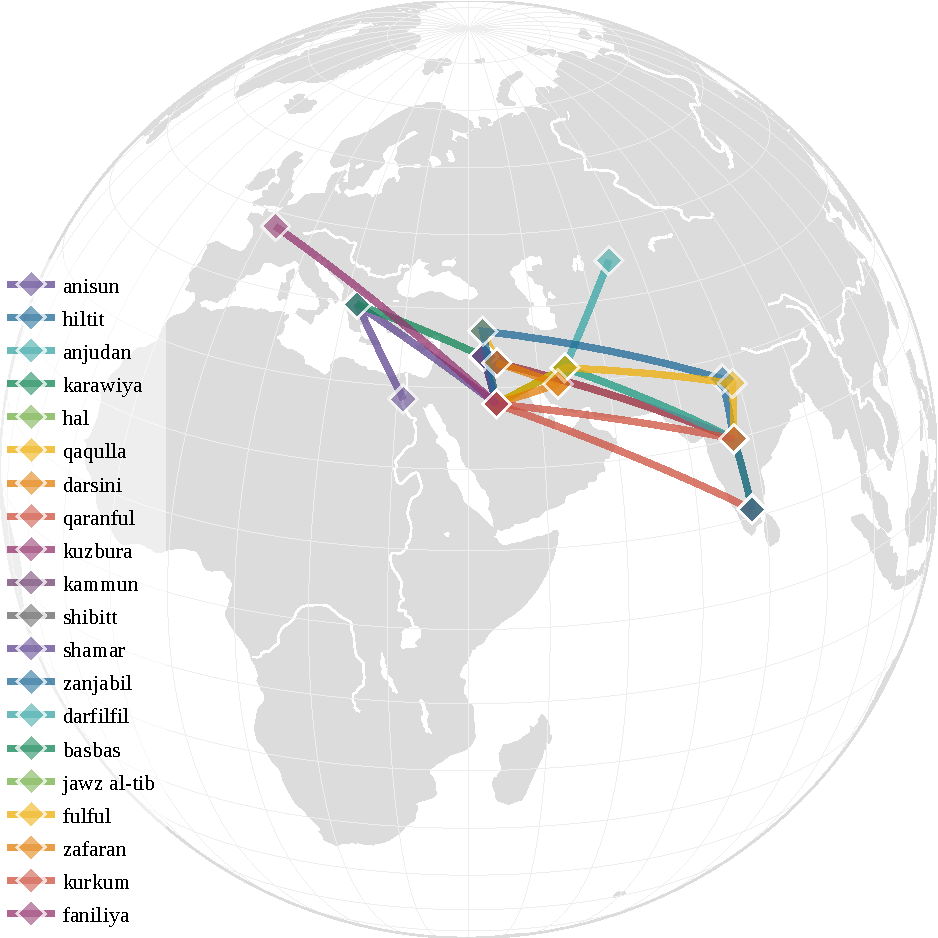
\includegraphics[width=\linewidth]{imgs/plots/diffusion_ar.pdf}
    \caption[The diffusion of spice terminology in Arabic.]{The diffusion of spice terminology in Arabic, focusing on loanwords and Wanderwörter. For a full interactive version, please visit \url{https://htmlpreview.github.io/?https://github.com/partigabor/phd-thesis-viz/blob/main/diffusion_ar.html}}
    \label{fig:diffusion_ar}
\end{figure}

Arabic loanwords in the spice domain reflect where the Arab merchants sourced their spices from; either overland via Persia or by sea from India (e.g., \textit{fulful} `pepper', \textit{dārṣīnī} `cinnamon', \textit{dārfilfil} `long pepper', etc.). Regional Semitic borrowings are also present, these include spices that originate relatively close to Arabia and the peoples of the region who knew and used them; e.g., \textit{kammūn}, \textit{shibitt} `dill', \textit{shamar} `fennel', all three traced back to Akkadian. Arabia represents a bridge in the spice trade between Europe and Asia, connecting the Orient and Occident during the peak of the spice trade starting from the \nth{6} century. In fact, the rise of Mecca, ``the cradle of Islam'' is known to have become properous due to the trade that lead ships to moor around the coast of Arabia, and turned caravans towards its flourishings trading posts with the ultimate goal of exchanging products for money with the merchants of the Mediterranean. The Arabs were so skilled traders that soon they managed the coastal trade in Indian ports as well, that represented the midway in the Indian Ocean trade network \autocite{parti_arab-indiai_2017}. 

\subsubsection{Spices in the Middle Kingdom: The Case of Chinese }

\begin{figure}[ht!]
  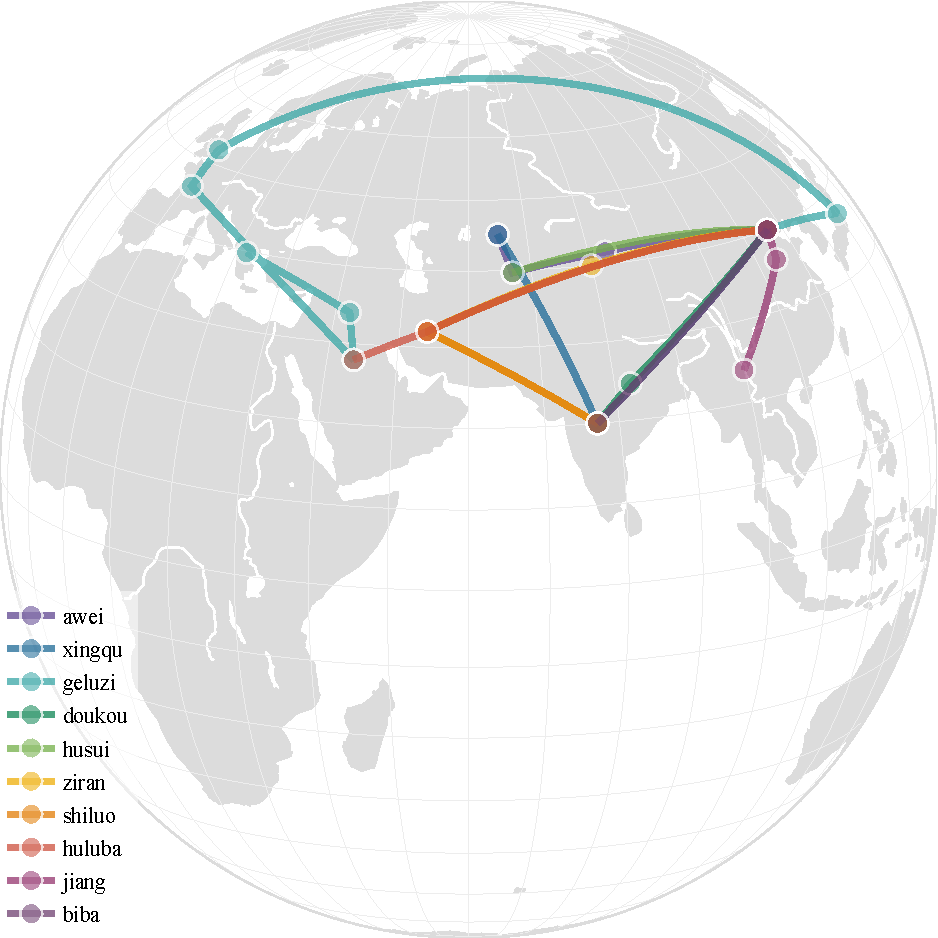
\includegraphics[width=\linewidth]{imgs/plots/diffusion_zh.pdf}
  \caption[The diffusion of spice terminology in Chinese.]{The diffusion of spice terminology in Chinese, focusing on loanwords and Wanderwörter. For a full interactive version, please visit \url{https://htmlpreview.github.io/?https://github.com/partigabor/phd-thesis-viz/blob/main/diffusion_zh.html}}
  \label{fig:diffusion_zh}
\end{figure}

Loanwords of the spice domain in Chinese mostly testify to the early---indirect---relationships with India and Central Asia through the Silk Roads and its peoples (see \textit{bibo} and \textit{xingqu} from Sanskrit, and \textit{awei}, \textit{husui}, and \textit{shiluo} via various iranian languages). \textit{Huluba} `fenugreek' is unquestionably a rendering of Arabic \textit{hulba}, most likely to arribe via Persian. More recent borrowings include \textit{duoxianggio} `allspice', a semantic translation of the English term, and \textit{geluzi} `caraway', that I traced to be a loan from Japanese who learned and coined this form from Western medicinal herbals. \textit{Ziran} is also a recent loanword from Uyghur.

It seems that Chinese loanwords represent spices that have arrived from a distance, India, Indo-China, and West Asia, and the Southeast Asian spices, such as nutmeg and cloves did receive Chinese names. A doubtful case is \textit{doukou} `cardamom', because it might represent an early Southeast Asian loan hidden by a partial phono-semantic matching, as it was discussed in \cref{sec:cardamom}.

\clearpage

\subsection{Temporal Trajectories: The Attestation of Spice Words}

After the investigation of how spice names reached English, Arabic, and Chinese on spatial trajectories, let us now look at how they have spread across time. One of the most exciting part of this thesis is the data that was collected regarding dates of attestation. In other words, I tried to find the earliest possible mentions for each spice, and then combine this information in a way that enables us to see the diffusion of spices span throughout the history of a language and culture. This information is a valuable indicator, as it shows the approximate times of the earliest contact and introduction of the materials. In essence, we can grasp the history of the spice trade in the words: when they arrived, which spices were the earliest to be recorded, and which ones make the latest additions to our vocabularies and spice cabinets. Here as well, from the nearly 360 names, I have used the selected few that---for lack of a better word---I marked with ``default''. To make the attestation visualizations easy to read, I only used the default terms, and a small number of historic terms that precede the contemporary default ones. This allows for a less packed and cleaner plot and offers a way to compare the attestations in the three languages. 

\begin{figure}[!ht]
  \centering
  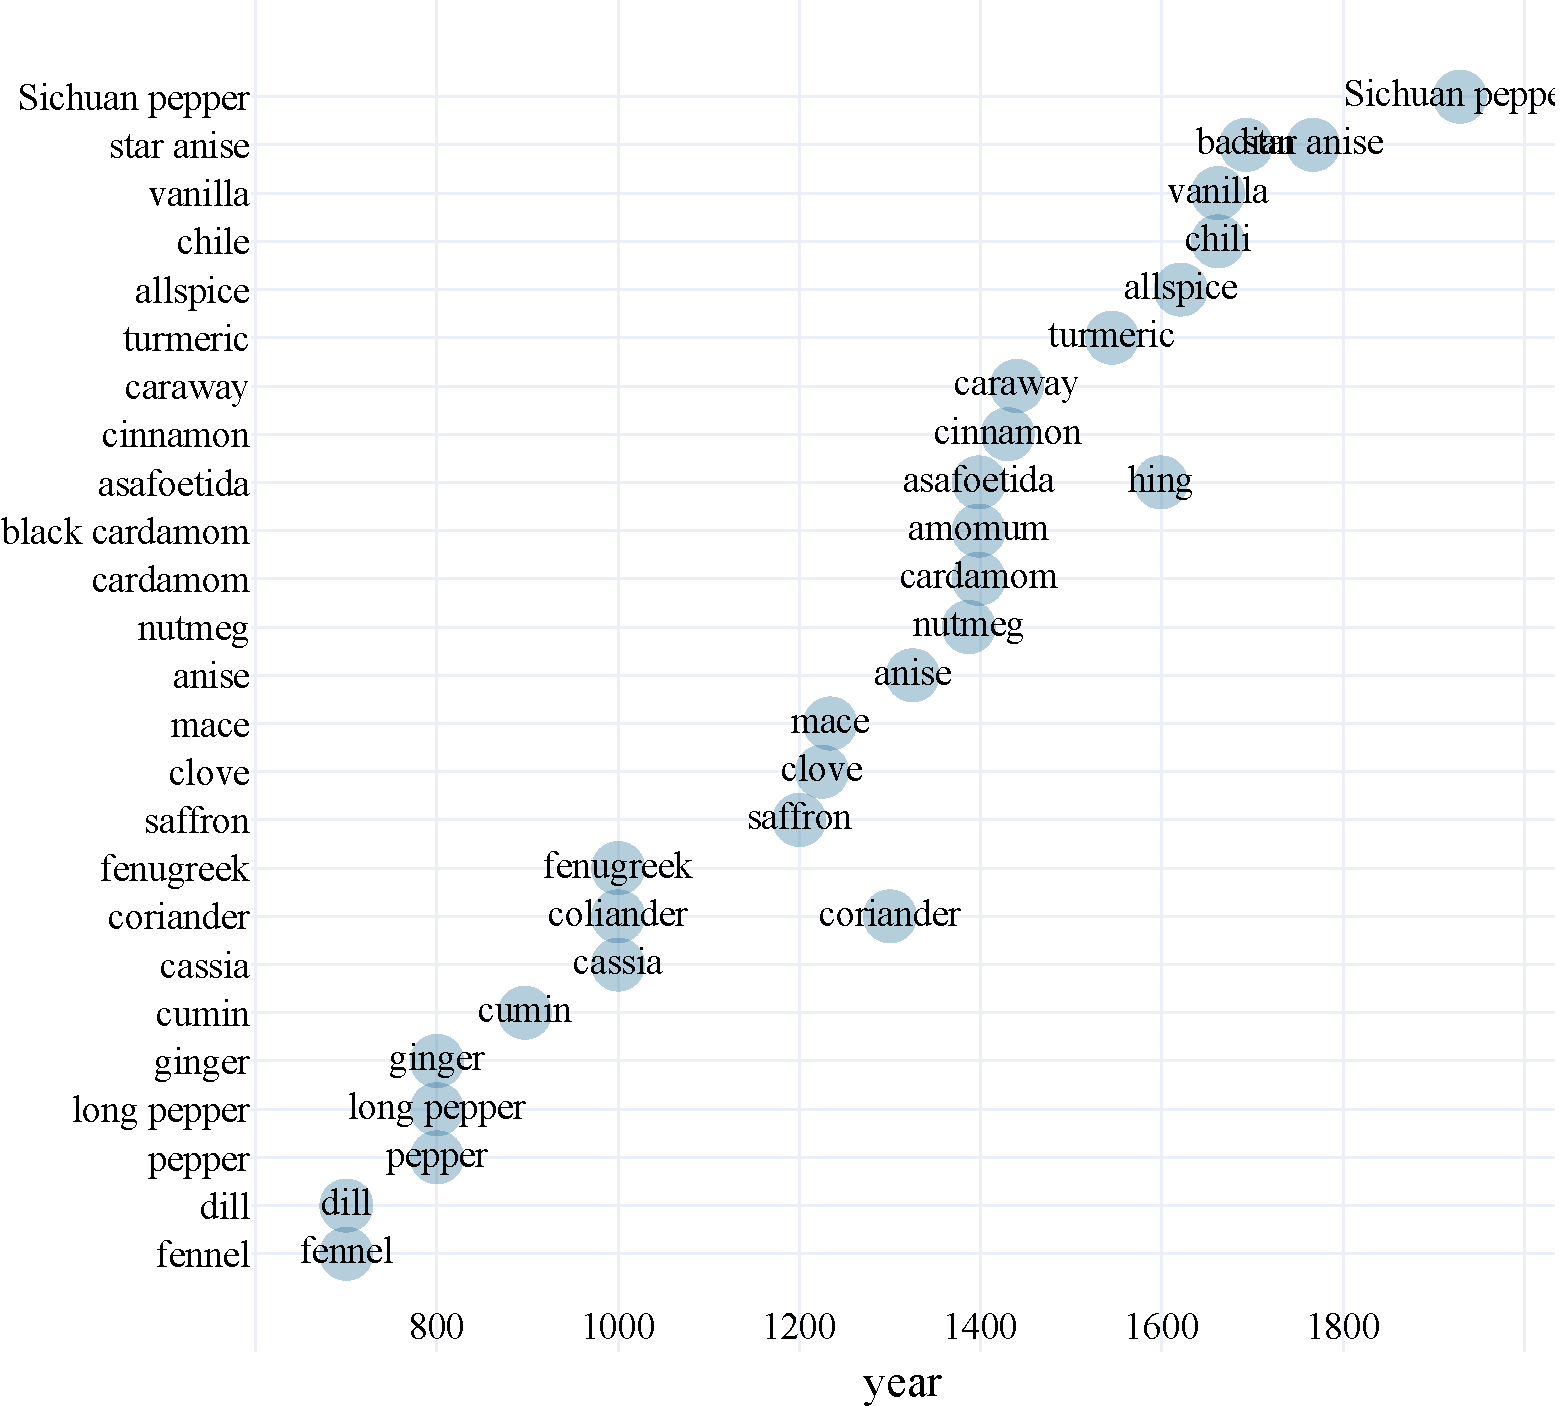
\includegraphics[width=\linewidth]{imgs/plots/attestation_en.pdf}
  \caption{Attestation timeline for spice terms in English.}
  \label{fig:attestation_en}
\end{figure}

\begin{figure}[!ht]
  \centering
  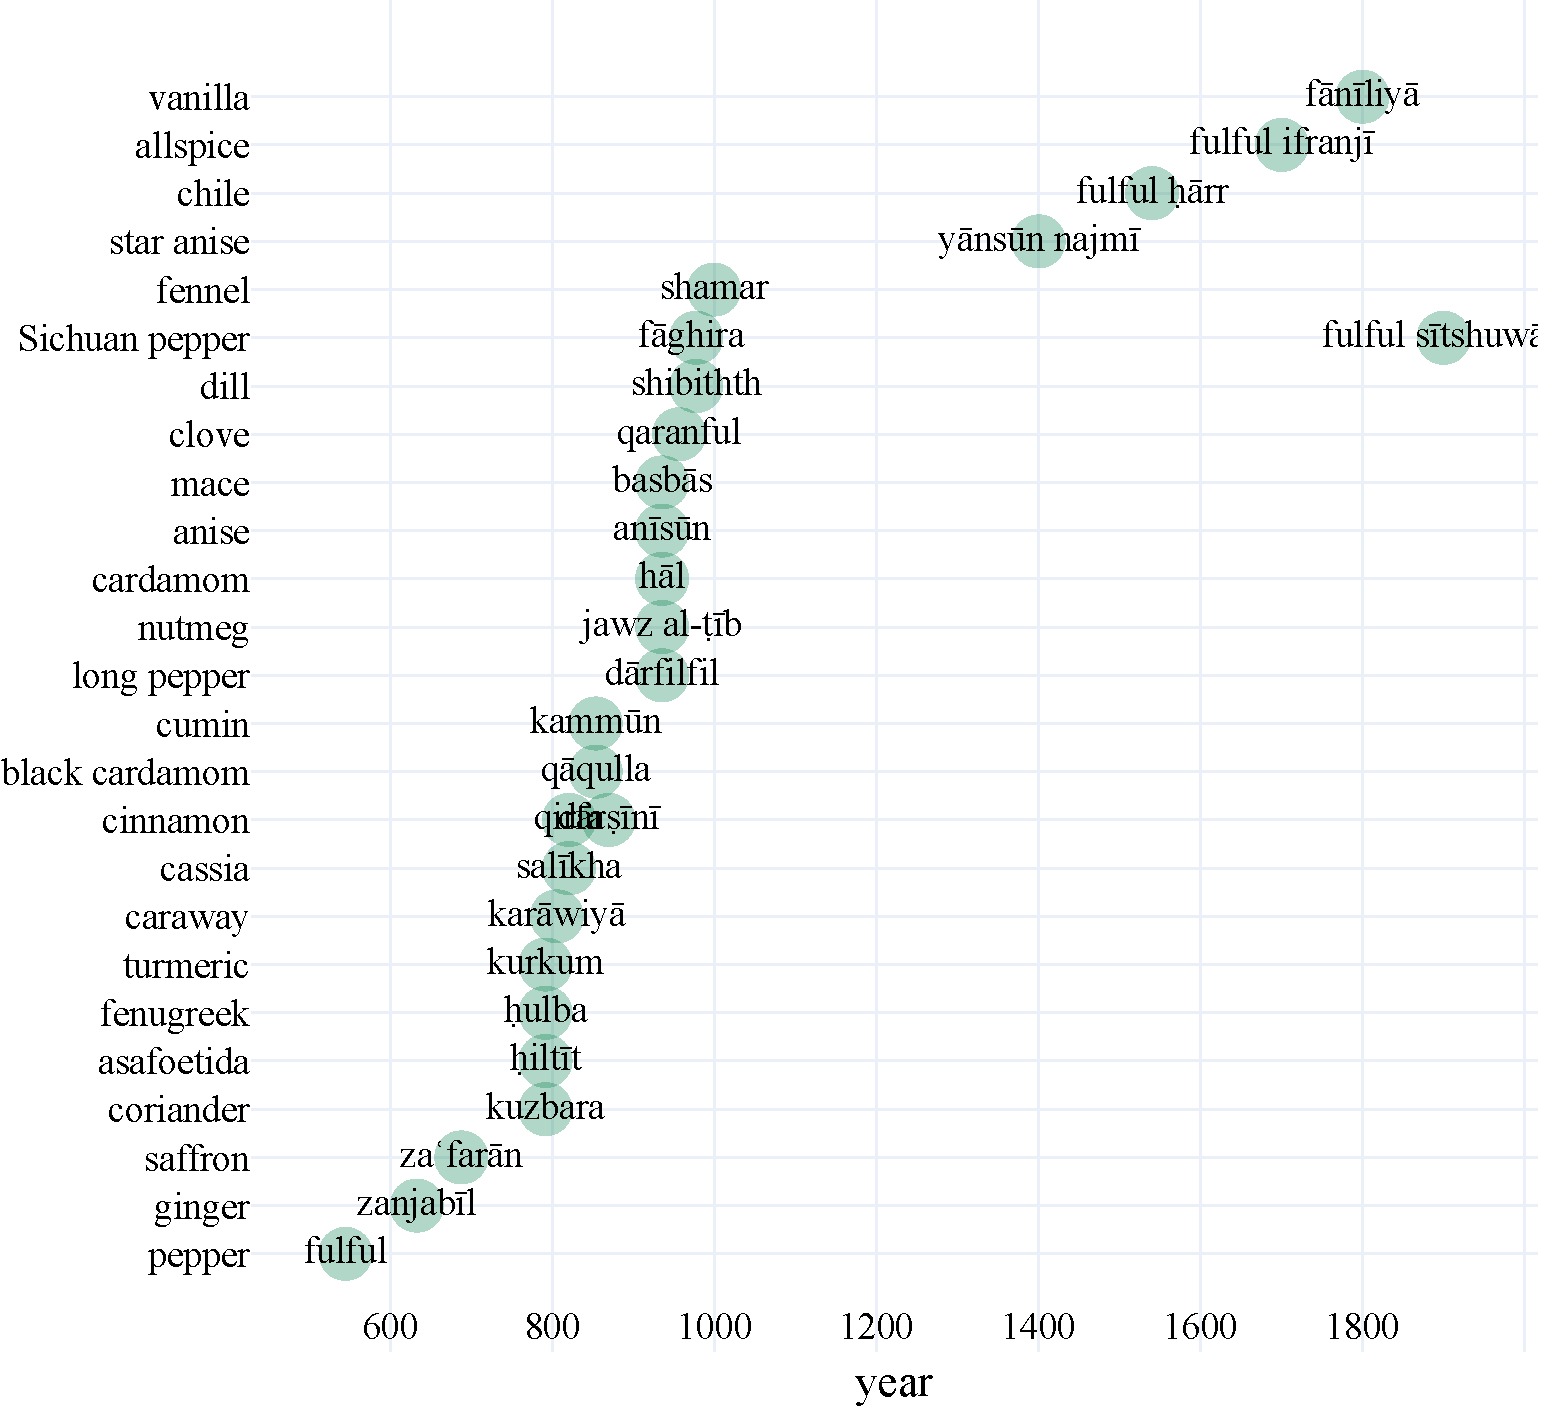
\includegraphics[width=\linewidth]{imgs/plots/attestation_ar.pdf}
  \caption{Attestation timeline for spice terms in Arabic.}
  \label{fig:attestation_ar}
\end{figure}

\begin{figure}[!ht]
  \centering
  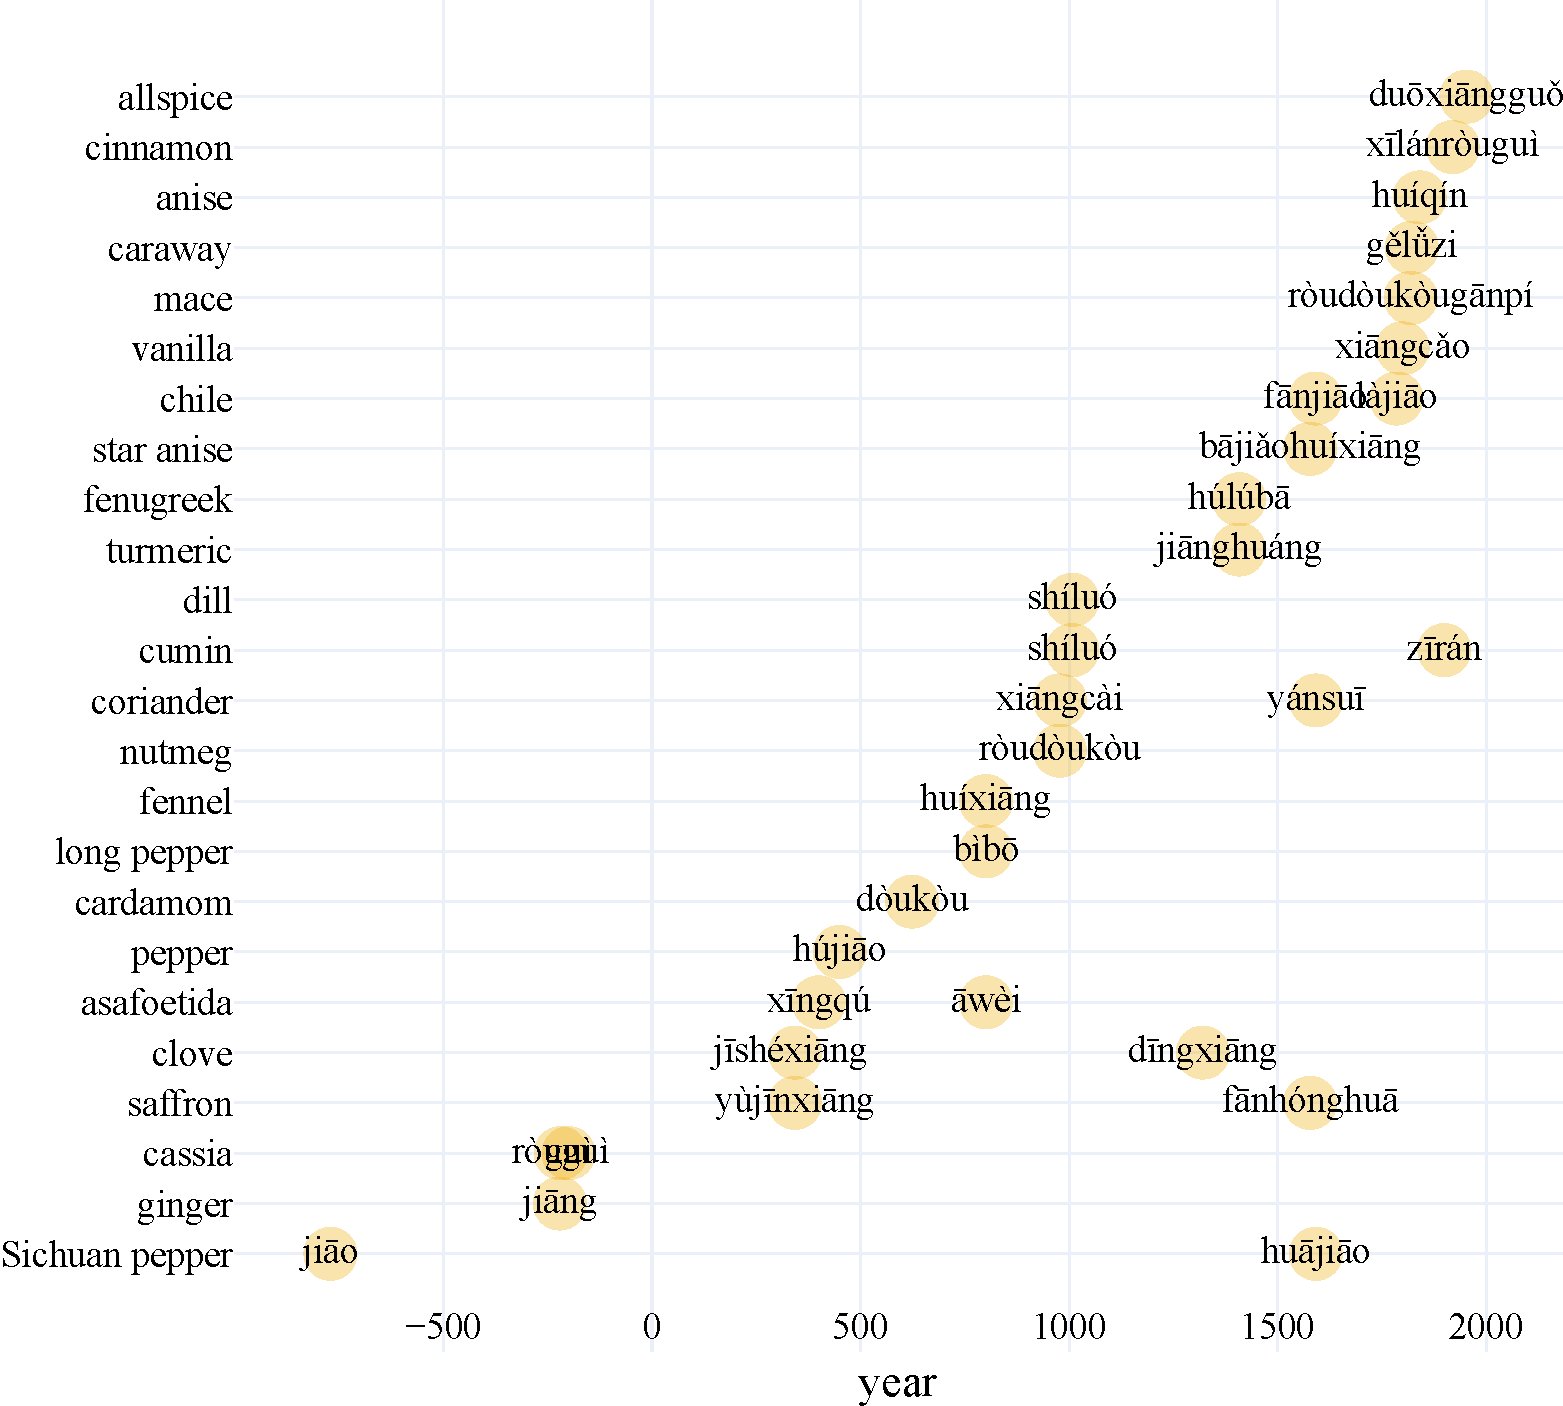
\includegraphics[width=\linewidth]{imgs/plots/attestation_zh.pdf}
  \caption{Attestation timeline for spice terms in Chinese.}
  \label{fig:attestation_zh}
\end{figure}

The following figures should give a bird's eye view of the history of the spice domain, and its mark on vocabulary. In \cref{fig:attestation_en,fig:attestation_ar,fig:attestation_zh}, you can see the timeline of the spice nomenclature language by language. Not surprisingly, these figures will show that the native spices that are to be found the closest to the homeland of the ancestors of English, Arabic, and Chinese speakers, have been recorded first. See dill and fennel in English, saffron and fenugreek in Arabic, and Sichuan pepper and cassia in Chinese. If we reflect back to the geographical origins of the spices (\cref{fig:spices_map}) the figures also show which are the earliest products of transnational trade, those that spread first despite their origins were distant and unknown to the early recipients. Primarily, these include pepper and ginger, which we already discussed were ideal candidates because of their resistance to long-haul transportation and hight scores of (biological) spreadability. 

In the final trilingual plot in \cref{fig:attestation_and_borrowing_compact} I have a produced a compact version of the same data, arranged by language. There is a chance to compare the main attestation periods for these items, and I added an accompanying histogram to better see which periods have seen the emergence of new spice words, indicating both flourishing periods of literature and trade. 

\begin{figure}[!ht]
  \centering
  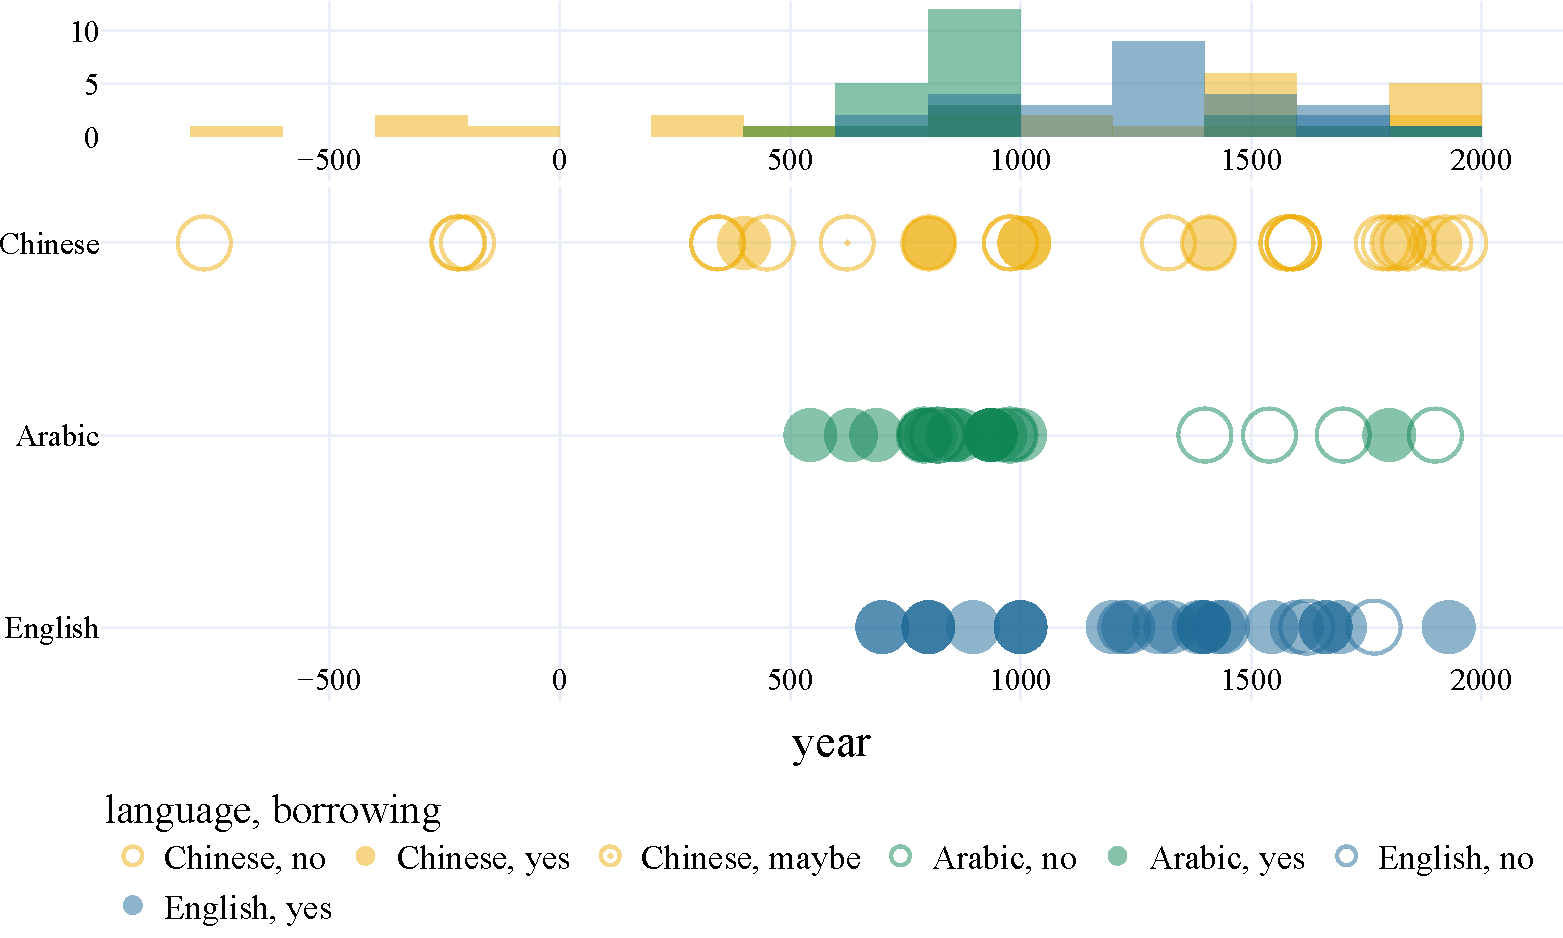
\includegraphics[width=\linewidth]{imgs/plots/attestation_and_borrowing_compact.pdf}
  \caption[Comparative timelines for attested spice terms, indicating borrowings.]{Comparative timelines for attested spice terms in English, Arabic, and Chinese, indicating borrowings. For a full interactive version, please visit \url{https://htmlpreview.github.io/?https://github.com/partigabor/phd-thesis-viz/blob/main/attestation_and_borrowing_compact.html}}
  \label{fig:attestation_and_borrowing_compact}
\end{figure}

Looking at \cref{fig:attestation_and_borrowing_compact}, we can observe a few trends off glance. First of all, it is clear that Chinese---the language with the longest literary tradition out of the three languages---has the earliest attested spice words, primarily \textit{jiao} `pepper', originally referring to the indigenous Sichuan pepper, but now also used to denote the black pepper and chili pepper especially. In this sense, \textit{jiao} is the equivalent of English \textit{pepper}, and Arabic \textit{fulful}. \textit{Jiao} is followed in time by \textit{gui} and \textit{rougui}, referring to the spice we know and use as cinnamon (but actually cassia), a tree native to the South of China, in the immediate proximity of the ancient Chinese heartland. As for \textit{jiang} `ginger'---also attested at a very early date---I have already mentioned the reasons for its early diffusion and consequent inclusion into the medicinal and culinary traditions of ancient people \textit{worldwide}. The attestation dates of other spices distribute evenly starting from the \nth4-{5} century, which marks the introduction of Buddhism into China from Central Asia along the Silk Roads, entering through the Gansu corridor. Besides monks carrying saffron, and asafoetida, we must not forget the many nomads and traveling traders, who likely introduced pepper as well (literally (nomadic) barbarian-pepper in Chinese), before the emergence of the Sogdians responsible for the introduction of many articles of trade during the Tang dynasty. 
%saffron  
The attestation of many spice names in the modern period is worth noting, these include spices that were known before but not distinguished (caraway seeds were not considered a separate spice from cumin, but were surely known in the Western Regions), or spices that were (are?) not used traditionally (allspice, anise, Ceylon cinnamon).

Secondly, there is an obvious jump in the attested Arabic terms in the \nth{8} century, which is considered the start of the Islamic Golden Age. During this time, science and literature flourished under the Abbasid caliph Harun al-Rashid, and the ``House of Wisdom''\footnote{The House of Wisdom (Arabic: \textit{Bayt al-Ḥikmah}) refers to a large library and/or academy famous for the voluminous translation work that produced an output of scientific literature from all sources and traditions including Greek, Roman, Persian, Indian, and the Arabic literature that built on and advanced the various sciences. Recently it has been suggested that the House of Wisdom was not an actual library but rather a metaphor referring to the active scientific community as a whole during early Abbasid dynasty. The library---if it existed---perished during the total destruction of Baghdad in 1258 by the hands of Hülegü and the Ilkhanid Mongols, thus little archeological evidence remains.} in Baghdad, the largest city in the world at the time \autocite{gutas_greek_1998}. It is worth noting that many of these terms became part of the Arabic vocabulary certainly much earlier than the attestation dates, but since the Arabic literary tradition begins with the compilation of the Quran (shortly after the death of Prophet Muhammad {ﷺ} in 632), we have little early documentary evidence. The earliest example would be from the \textit{Jahiliyya}\footnote{Literally meaning `ignorance', this term refers to the pre-Islamic period of Arabia.} era poet Imru' l-Qays, whose poetry features the word \textit{fulful/filfil} `pepper'.

Thirdly, English features a set of spices that were attested in Old English, many known to the Romans since Biblical times, such as...
But we can also see the time when Europe bacame aquantied with further oriental spices after the Crusades, when the westerners who who have acquired a taste for lavish Eastern flavors started to bring them home.

The next trivial step is to add the feature of borrowings to the plot, to see chronologically which terms were borrowed, and which are native inventions. 
% Loanwords and \glspl{wanderwort} frequent the spice spice nomenclature in many languages




\subsection{The Donor Languages}

% \begin{wrapfigure}{O}{0.66\textwidth}
%   \vspace{-\baselineskip}
%   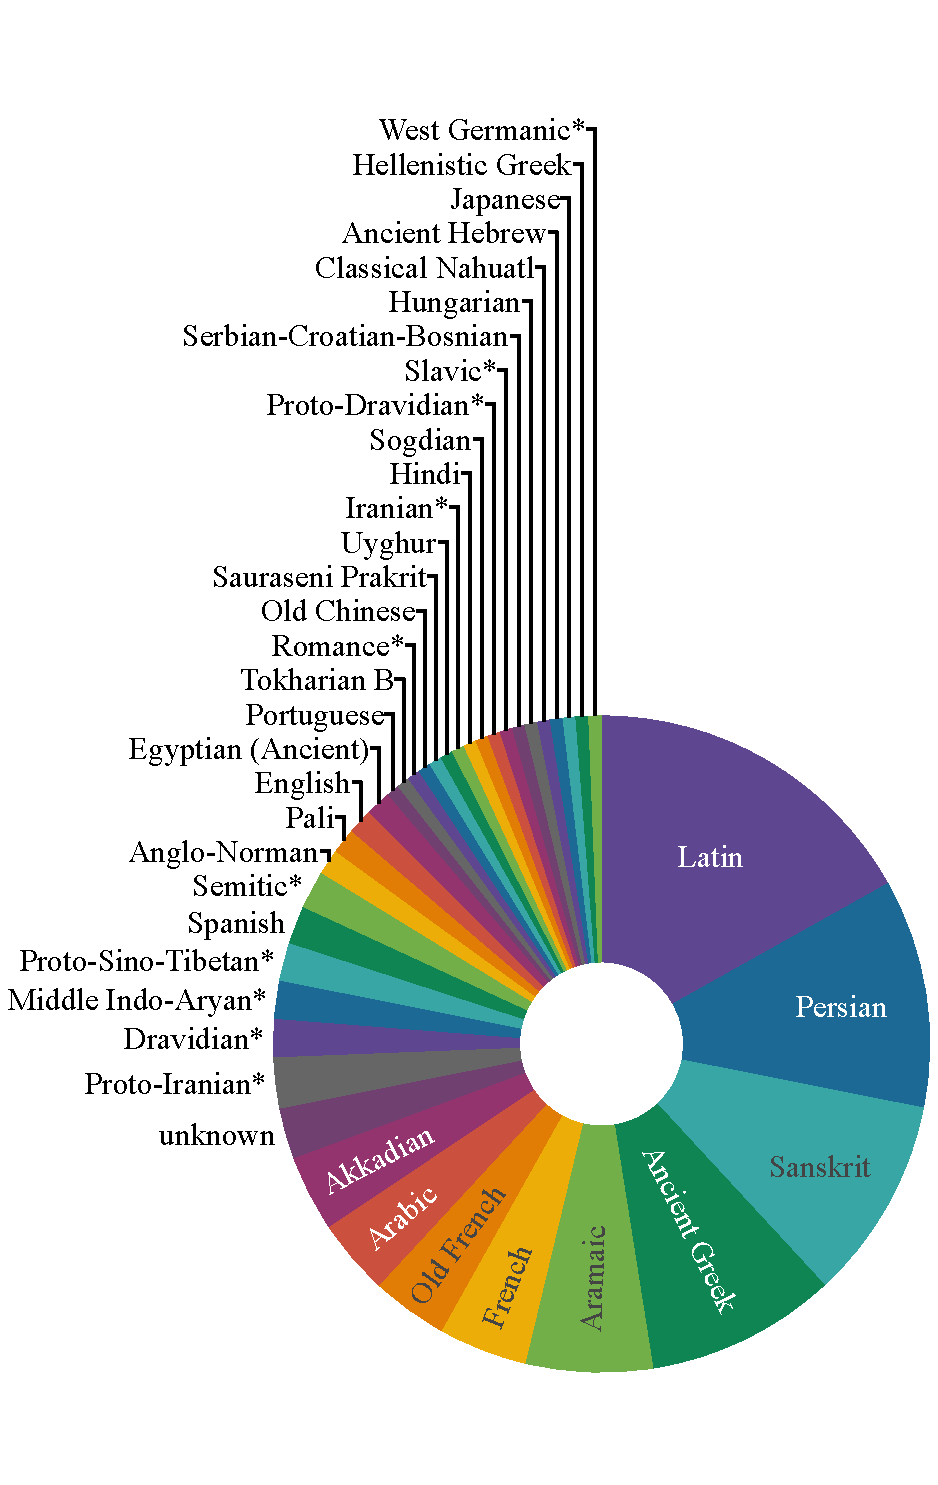
\includegraphics[width=0.66\textwidth]{imgs/plots/donors_pie.pdf}
%   \caption{All identified donor languages of loanwords in the spice domain.}
%   \label{fig:donor_pie}
% \end{wrapfigure}

So who loaned these words? Which languages and civilizations are responsible for transmitting, transmutating, and disseminating the terms of the spice domain? From the etymological dataset, I have extracted the \textit{participating} languages. In order of their frequency, they are: Latin, Sanskrit, Persian, Ancient Greek, Aramaic, French, Akkadian, Old French, Arabic, Proto-Iranian*, Unknown, Middle Indo-Aryan*, Semitic*, Dravidian*, Iranian*, Anglo-Norman, Hungarian, Spanish, English, Pali, Egyptian (Ancient), Proto-Dravidian*, Uyghur, Turkic*, West Germanic*, Romance*, Proto-Sino-Tibetan*, Old Chinese, Old Tamil, Sauraseni Prakrit, Late Latin, Old English, Middle Chinese, Hindi, Tokharian B, Sogdian, Slavic*, Serbian-Croatian-Bosnian, Japanese, Classical Nahuatl, Hellenistic Greek, Ancient Hebrew, and Mandarin Chinese. Language families/branches, and proto languages are marked by an asterisk.

% \cref{fig:donor_pie} is an illustration of these languages.

To give this batch of information some meaning, I have broken down this data according to our three reference languages, English, Arabic, and Chinese. You can consult this in \cref{fig:donor_bar}. This bar chart shows the top 5 languages that have played a role in \textit{carrying} loanwords of the spice domain, at any given stage, wheter being the source, or a transmitting language. Speaking of source, \cref{fig:source_bar} shows the top 5 source languages of the loanwords of the spice domain.

\begin{figure}[!ht]
  \centering
  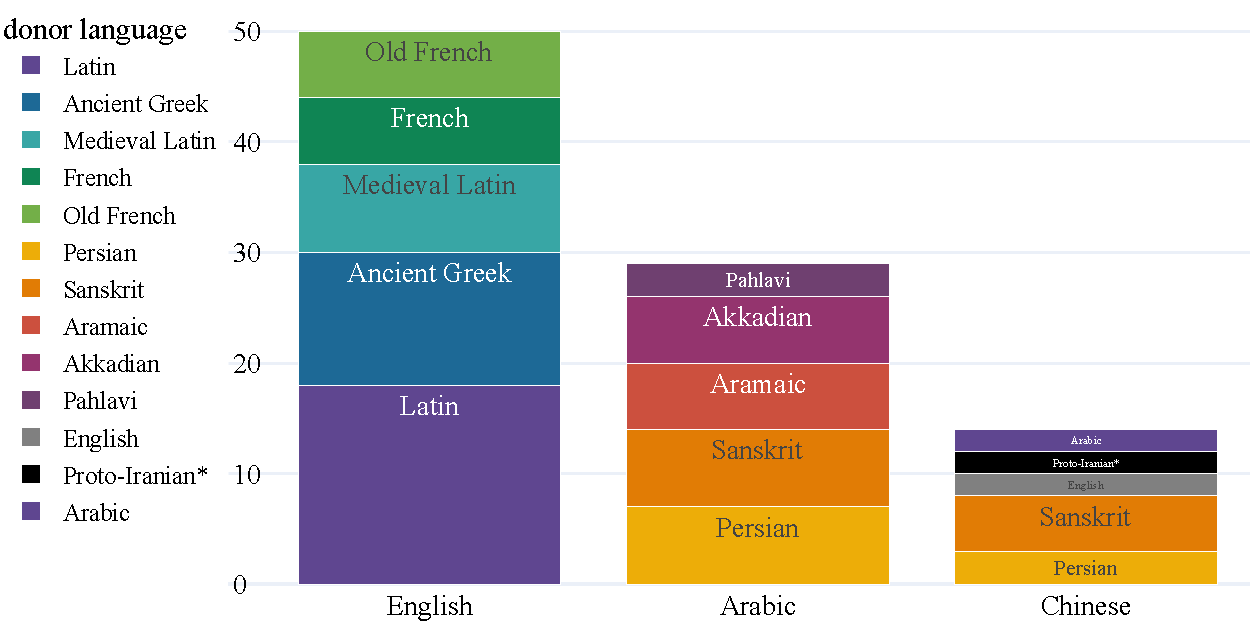
\includegraphics[width=\linewidth]{imgs/plots/donor_bar.pdf}
  \caption{Top donor languages of English, Arabic, and Chinese loanwords in the spice domain.}
  \label{fig:donor_bar}
\end{figure}

\begin{figure}[!ht]
  \centering
  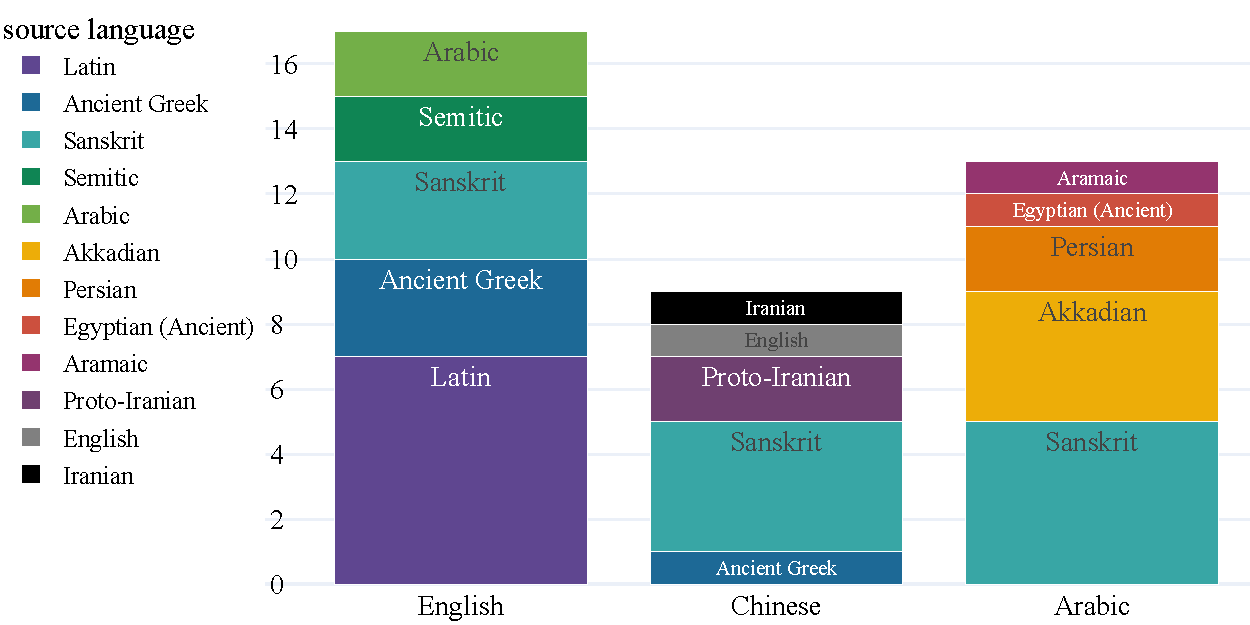
\includegraphics[width=\linewidth]{imgs/plots/source_bar.pdf}
  \caption{Top source languages of English, Arabic, and Chinese loanwords in the spice domain.}
  \label{fig:source_bar}
\end{figure}




